Первым экспериментом было решено провести сравнения показателей метрик HOTA, MOTA и IDF1 от размера сети детектора на двух различных размерах изображений. Это исследование поможет определить, насколько значителен вклад увеличения сети детектора и размера изображения. 

Для проведения экспериментов было произведено вычисление показателей качества на наборе данных MOT17 с различными конфигурациями. Результаты исследования представлены на рисунках \ref{fig:yolo_ByteTrack}-\ref{fig:yolo_ImprAssOC}.

По графикам видно, что в целом самая маленькая модель yolov8n на размере изображения 512 на 512 работает по качеству сопоставимо с самой большой yolov8x на размере изображений 312 на 312. 
Более точно числа представлены для сравнения в таблицах \ref{tab:mean_hota_yolo_size} - \ref{tab:mean_idf1_yolo_size}.

\begin{figure}[ht]
    \centering
    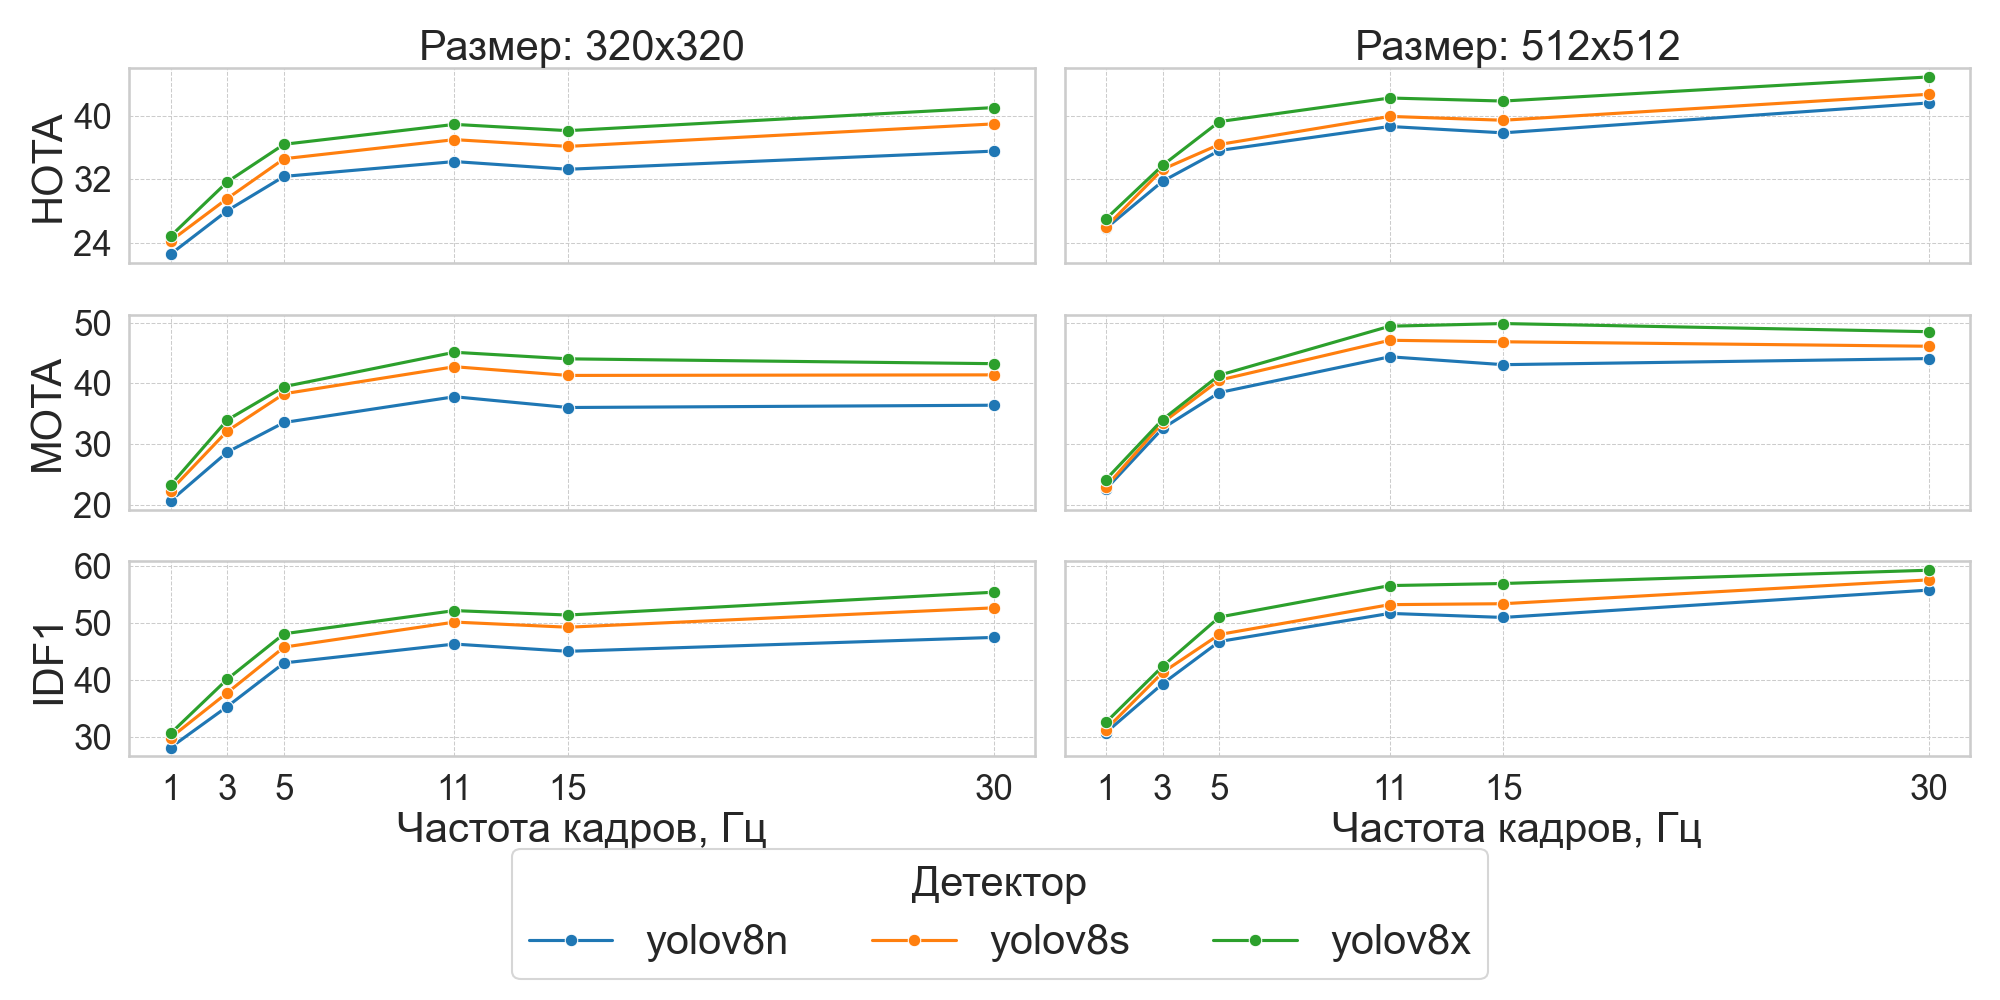
\includegraphics[width=1\textwidth]{plots/yolo_size_vs_metric/ByteTrack.png}
    \caption{График зависимости метрик HOTA, MOTA и IDF1 от размера сети детектора для алгоритма ByteTrack}
    \label{fig:yolo_ByteTrack}
\end{figure}

\begin{figure}[ht]
    \centering
    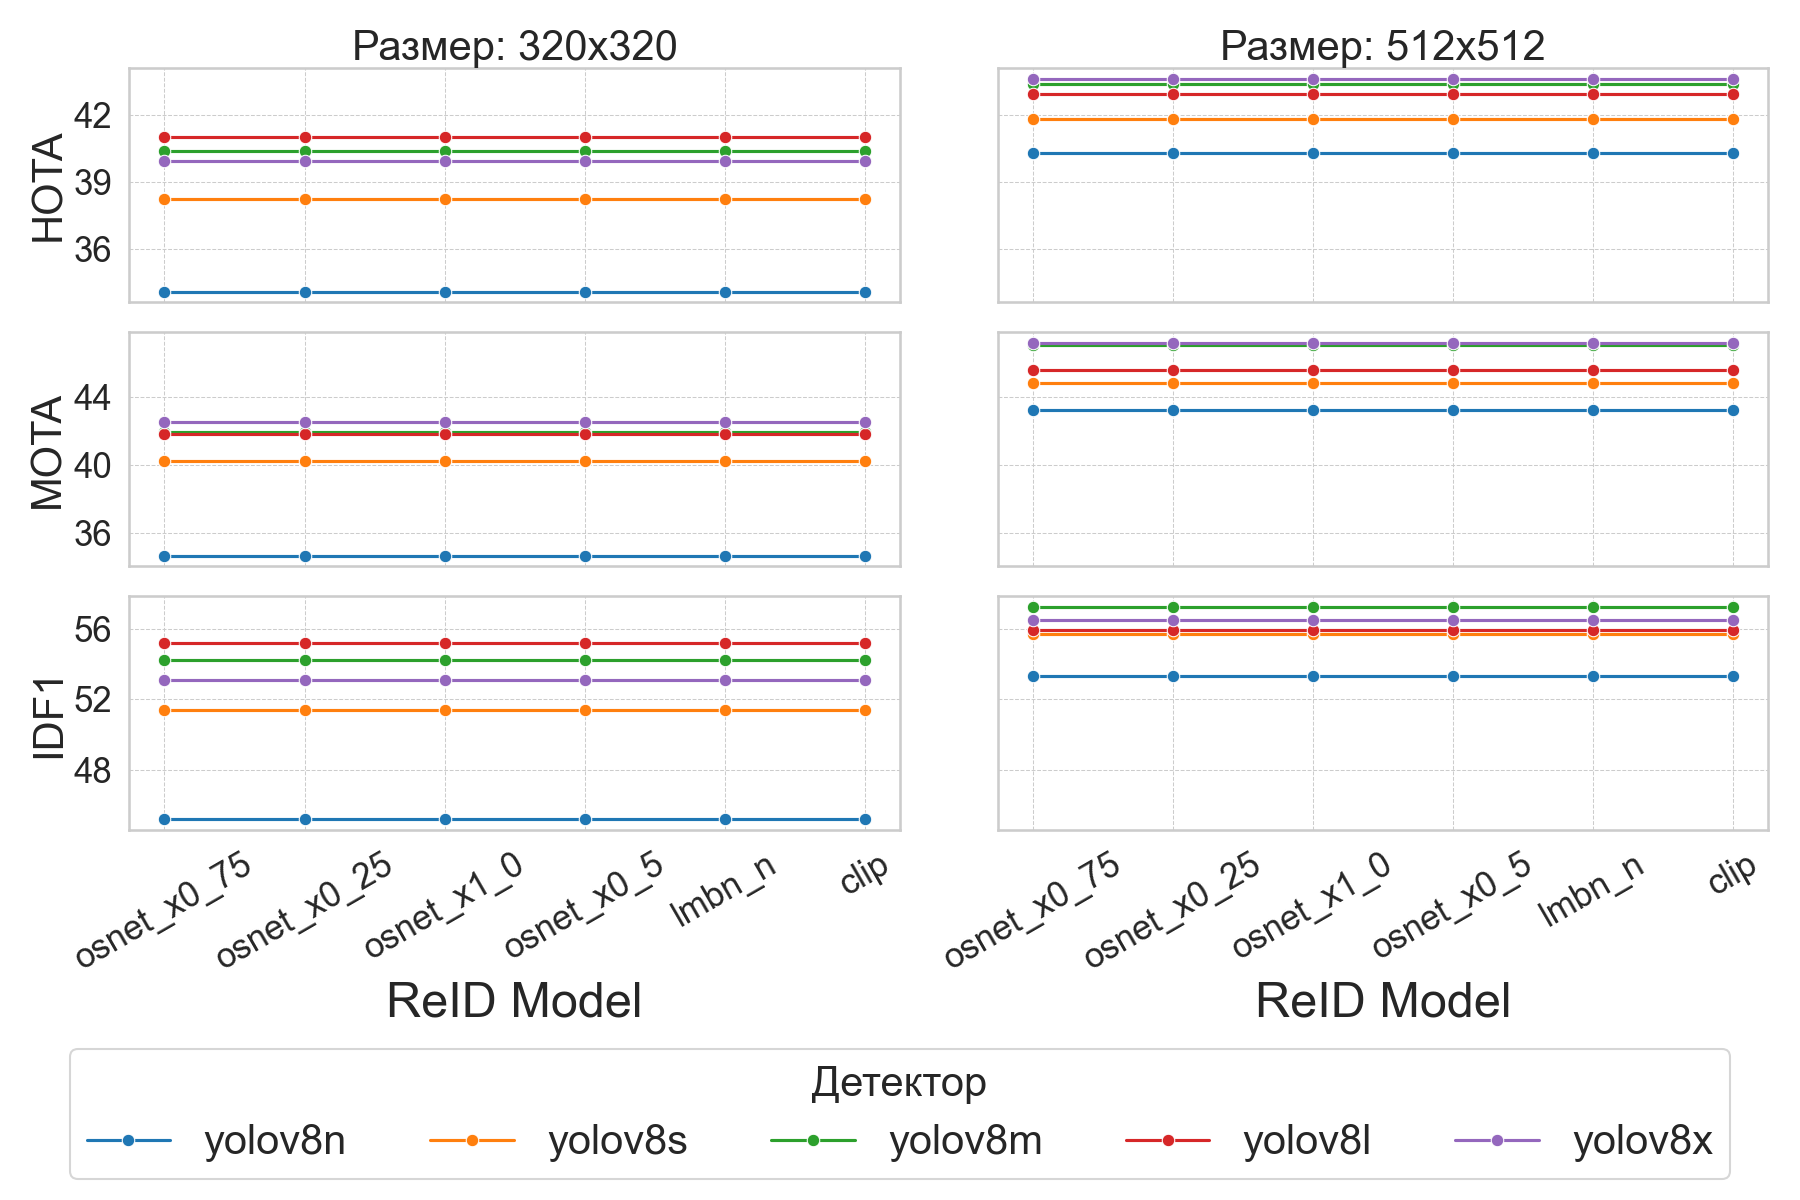
\includegraphics[width=1\textwidth]{plots/yolo_size_vs_metric/OC-SORT.png}
    \caption{График зависимости метрик HOTA, MOTA и IDF1 от размера сети детектора для алгоритма OC-SORT}
    \label{fig:yolo_OC-SORT}
\end{figure}

\begin{figure}[ht]
    \centering
    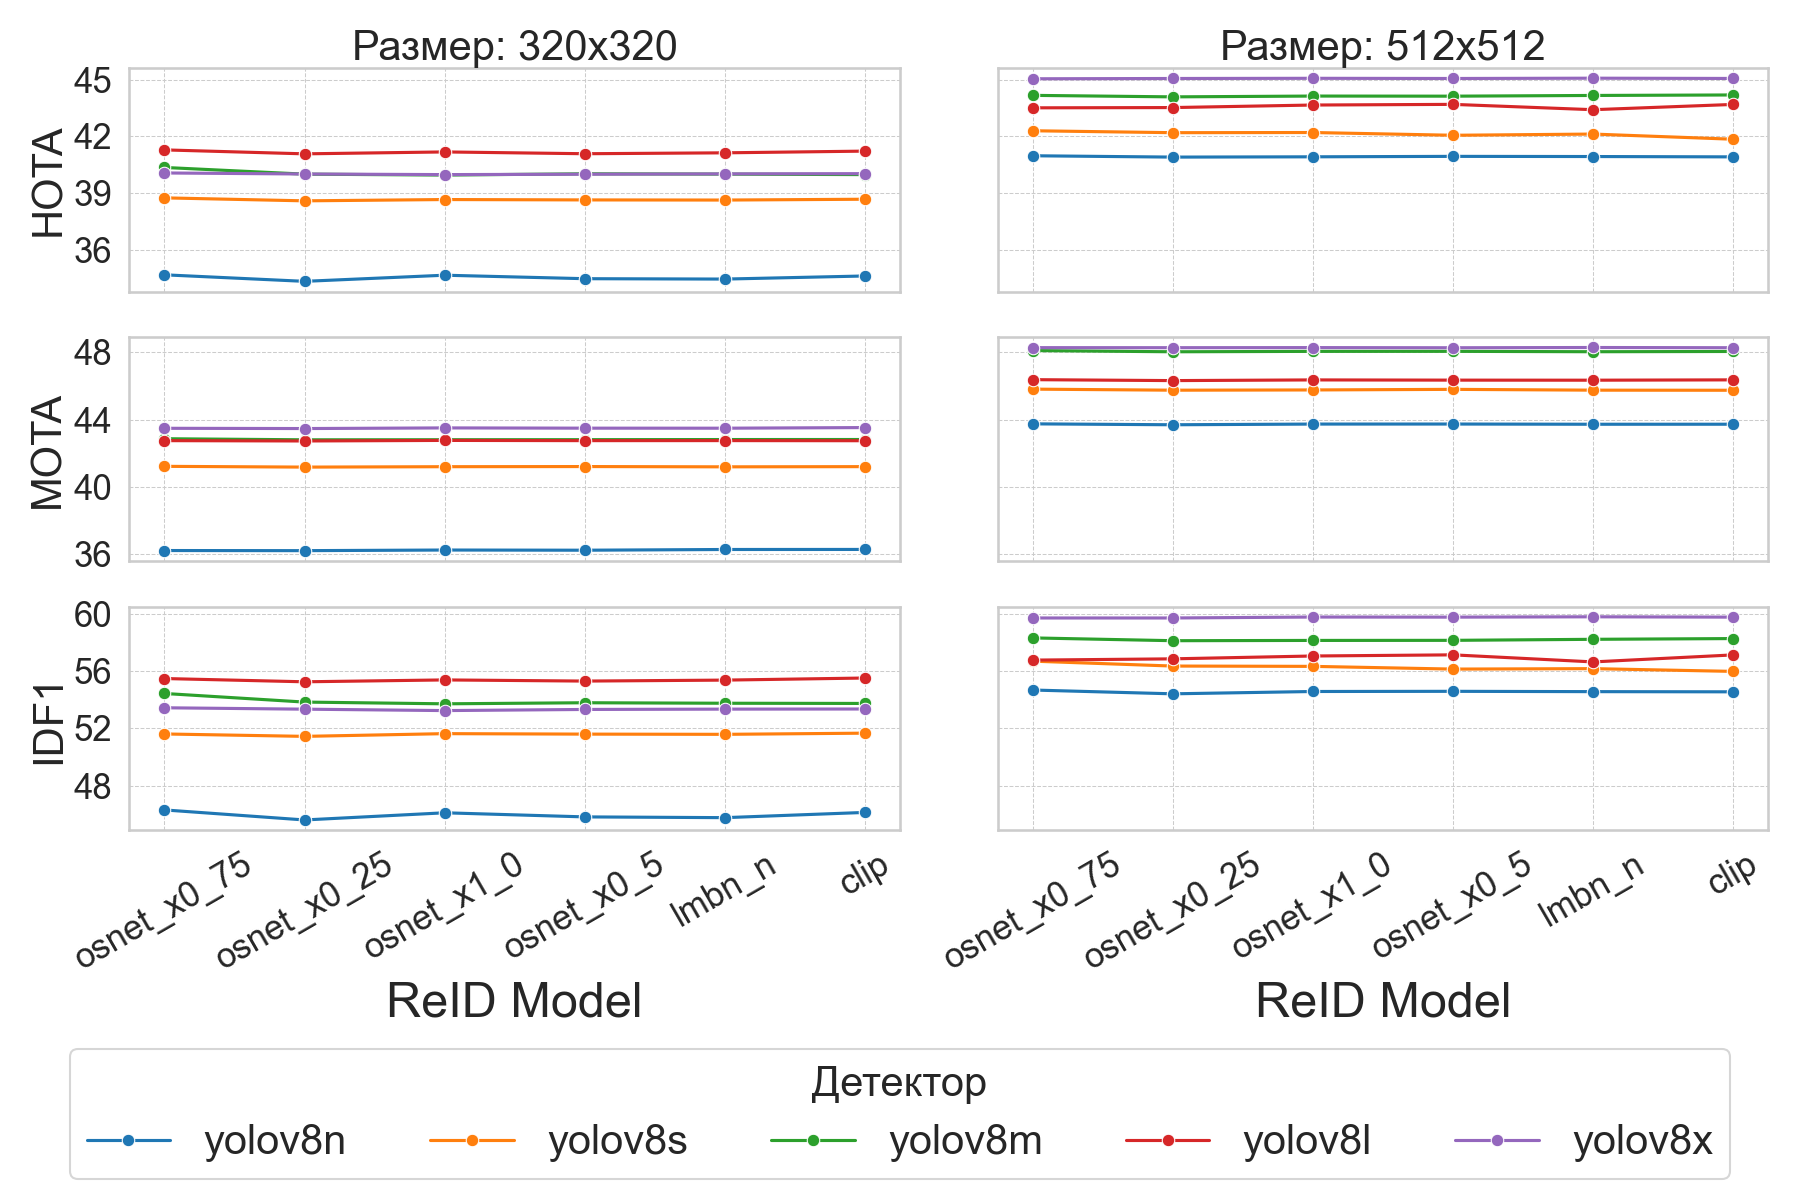
\includegraphics[width=1\textwidth]{plots/yolo_size_vs_metric/Deep OC-SORT.png}
    \caption{График зависимости метрик HOTA, MOTA и IDF1 от размера сети детектора для алгоритма Deep OC-SORT}
    \label{fig:yolo_Deep OC-SORT}
\end{figure}

\begin{figure}[ht]
    \centering
    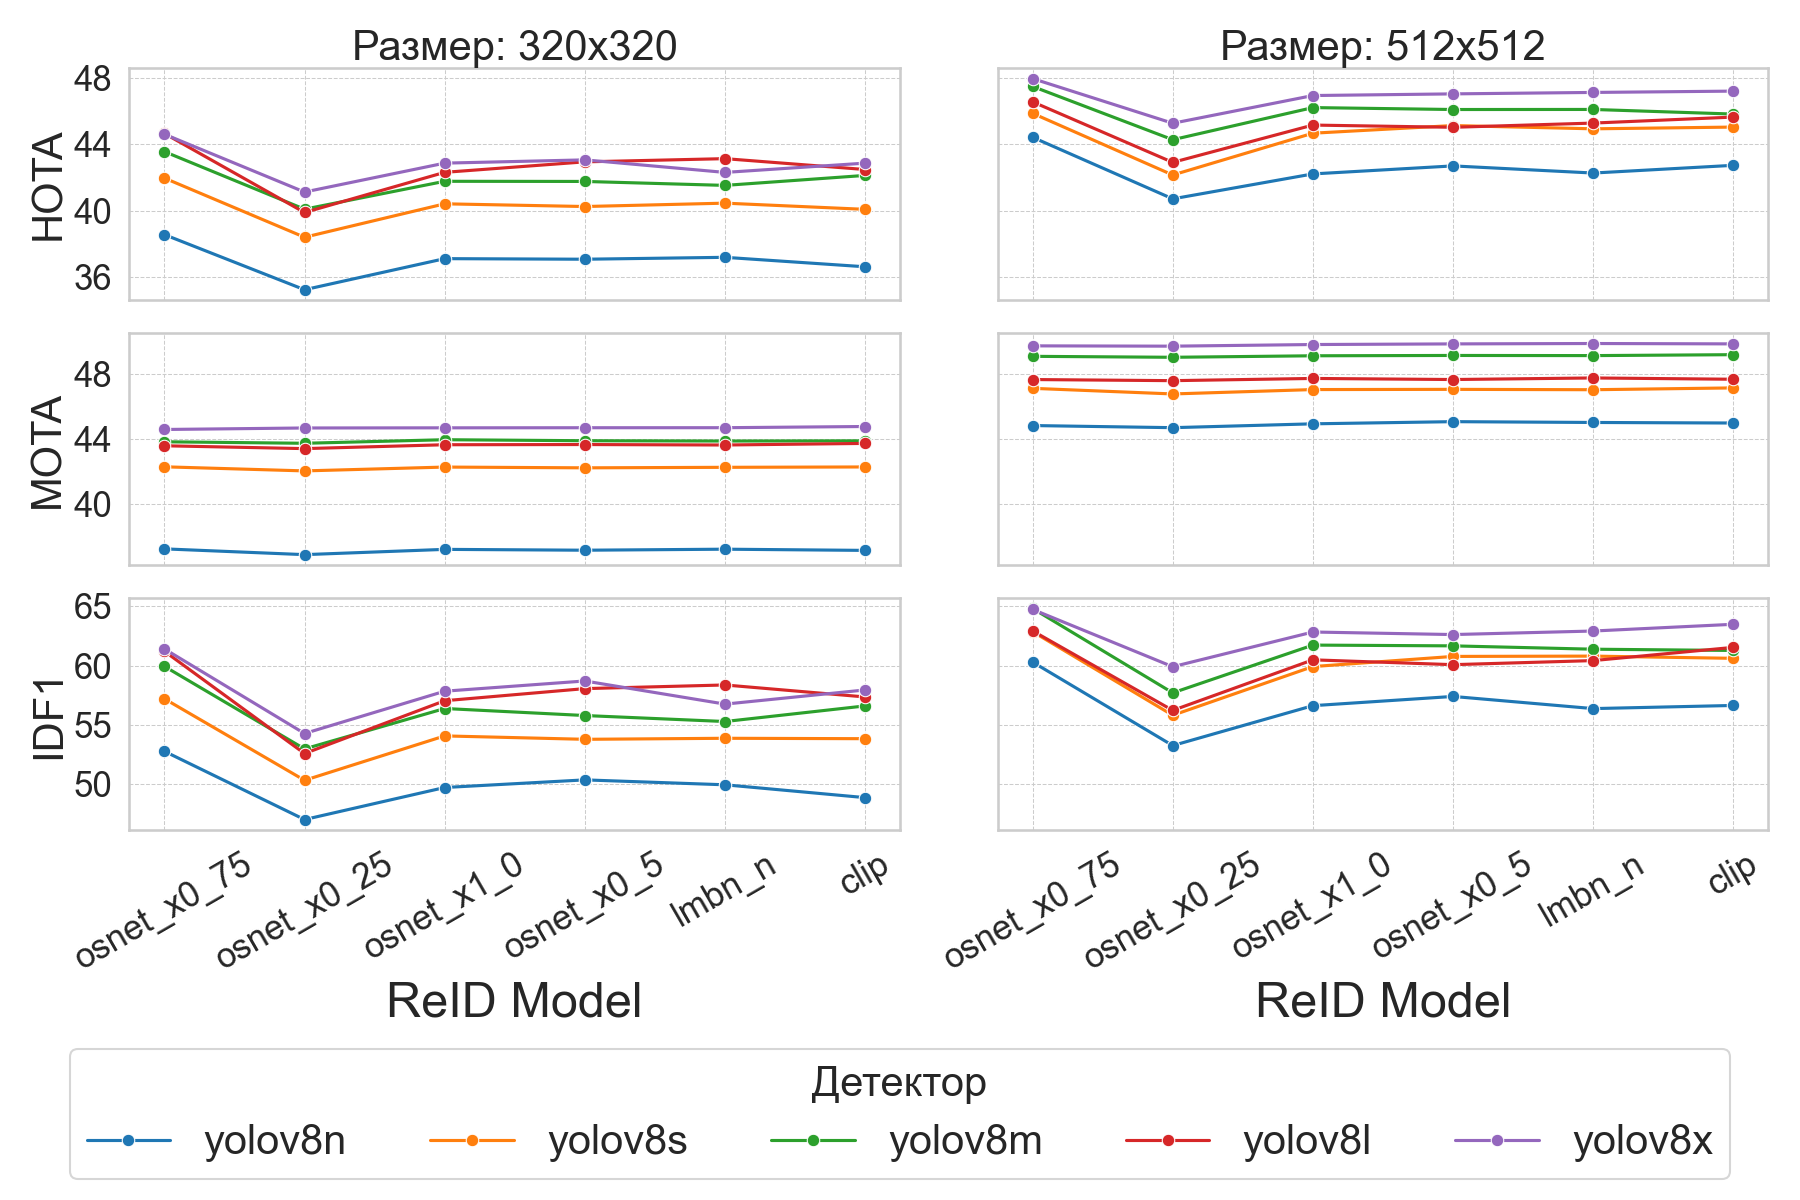
\includegraphics[width=1\textwidth]{plots/yolo_size_vs_metric/StrongSORT.png}
    \caption{График зависимости метрик HOTA, MOTA и IDF1 от размера сети детектора для алгоритма StrongSORT}
    \label{fig:yolo_StrongSORT}
\end{figure}

\begin{figure}[ht]
    \centering
    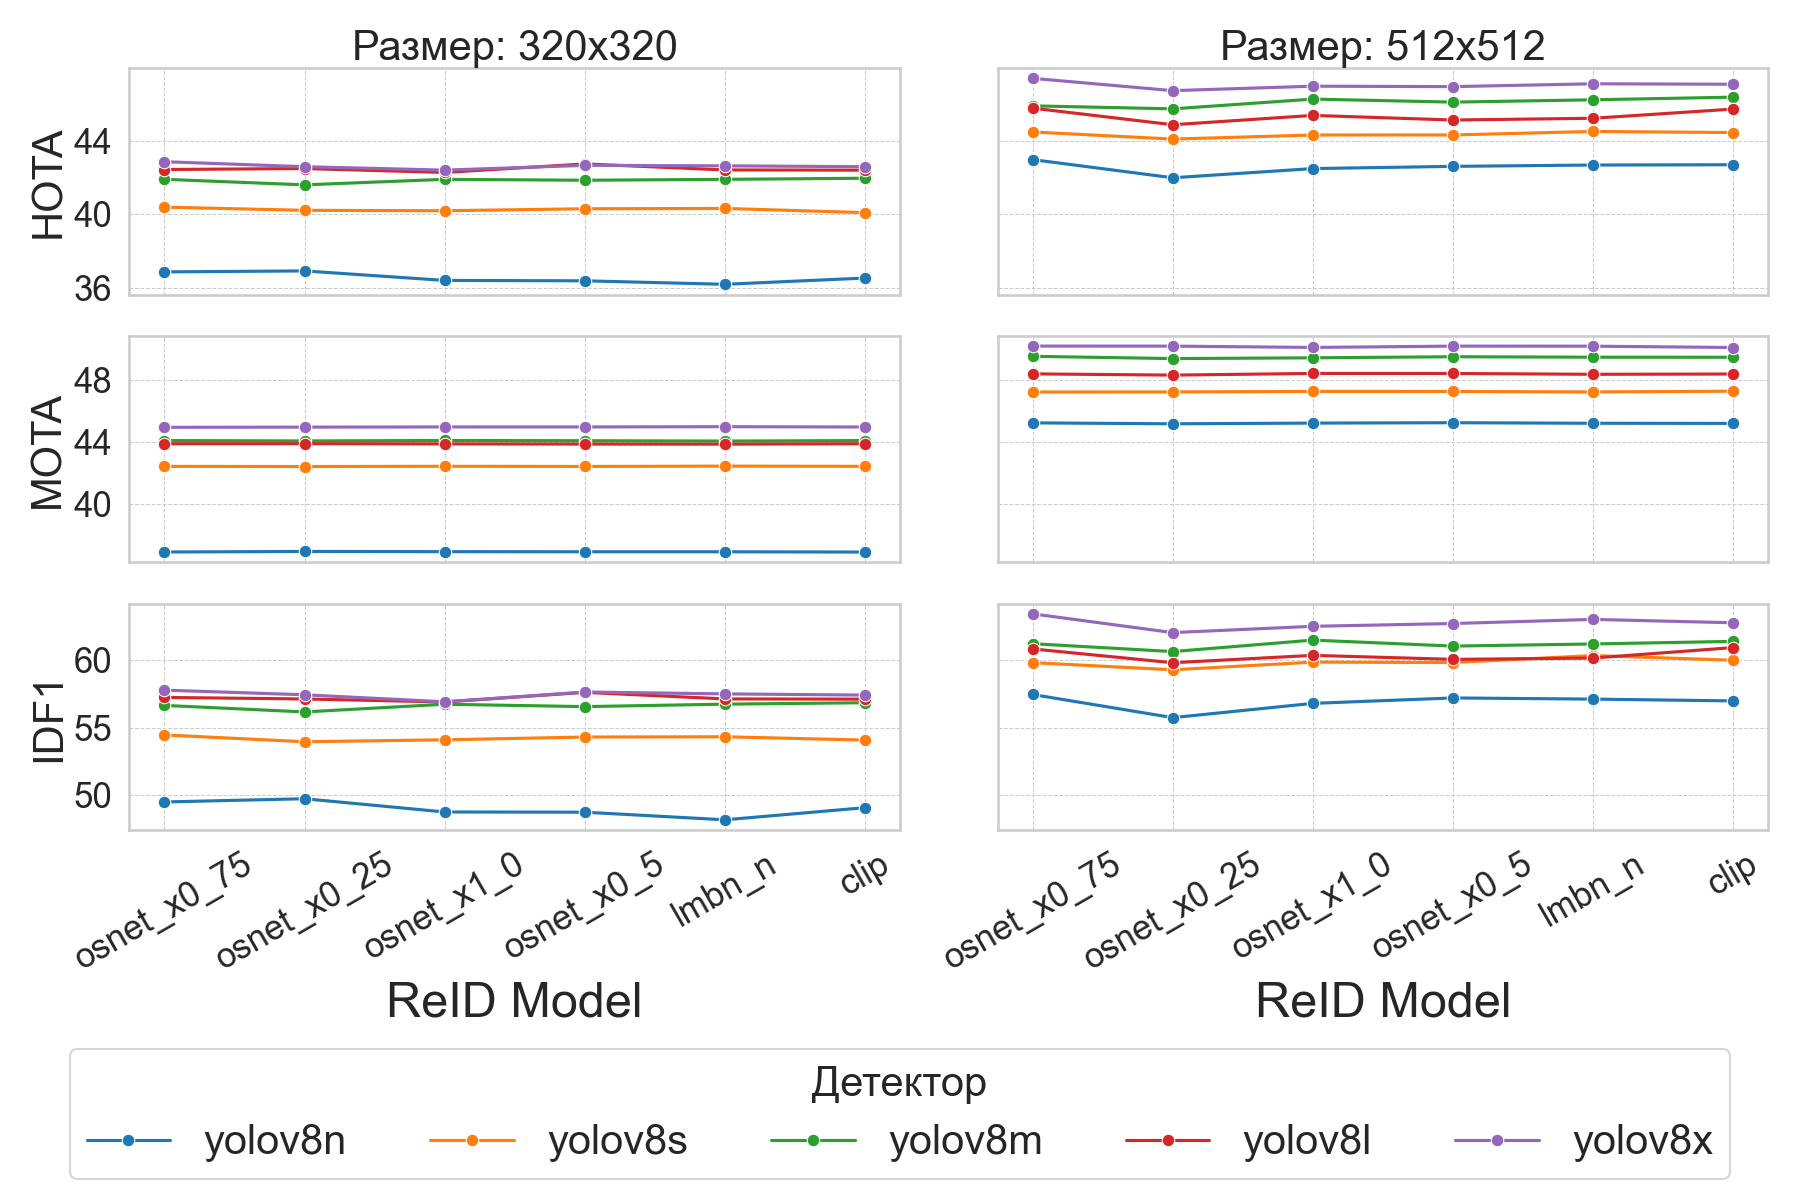
\includegraphics[width=1\textwidth]{plots/yolo_size_vs_metric/BoT-SORT.png}
    \caption{График зависимости метрик HOTA, MOTA и IDF1 от размера сети детектора для алгоритма BoT-SORT}
    \label{fig:yolo_BoT-SORT}
\end{figure}

\begin{figure}[ht]
    \centering
    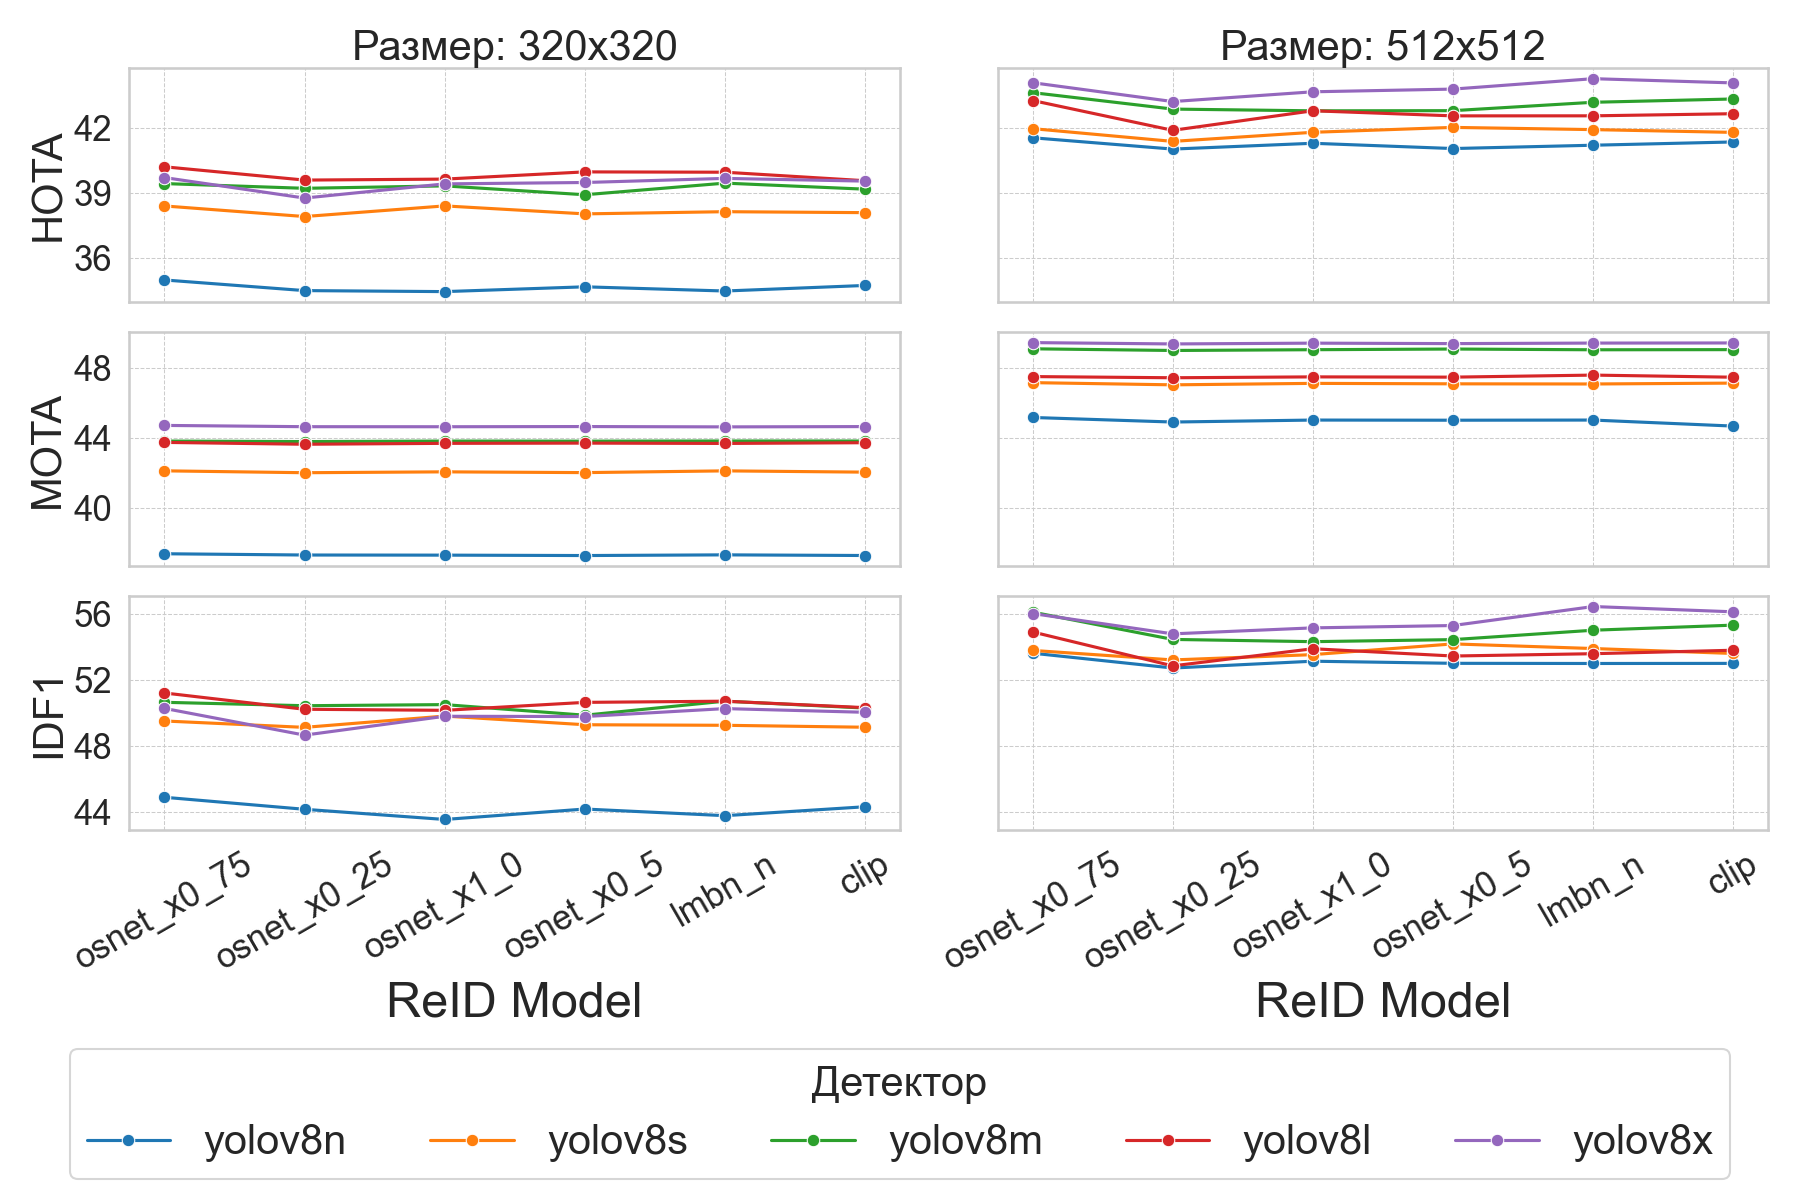
\includegraphics[width=1\textwidth]{plots/yolo_size_vs_metric/ImprAssOC.png}
    \caption{График зависимости метрик HOTA, MOTA и IDF1 от размера сети детектора для алгоритма ImprAssOC}
    \label{fig:yolo_ImprAssOC}
\end{figure}
\FloatBarrier
\begin{table}[htbp]

\caption{Среднее значение метрики HOTA для yolov8n и yolov8x}
\label{tab:mean_hota_yolo_size}
\centering
\begin{tabular}{lrrrr}
 & \multicolumn{2}{c}{320} & \multicolumn{2}{c}{512} \\
  & yolov8n & yolov8x & yolov8n & yolov8x \\
\midrule
BoT-SORT & 32.8 & 38.1 & 37.6 & 41.7 \\
ByteTrack & 31.0 & 35.2 & 35.2 & 38.2 \\
Deep OC-SORT & 30.6 & 35.1 & 35.4 & 38.9 \\
ImprAssOC & 34.0 & 38.3 & 38.8 & 42.0 \\
OC-SORT & 28.8 & 33.2 & 33.7 & 37.0 \\
StrongSORT & 34.5 & 39.3 & 38.9 & 42.7 \\
\bottomrule
\end{tabular}\end{table}
\begin{table}[htbp]

\caption{Среднее значение метрики MOTA для yolov8n и yolov8x}
\label{tab:mean_mota_yolo_size}
\centering
\begin{tabular}{lrrrr}
 & \multicolumn{2}{c}{320} & \multicolumn{2}{c}{512} \\
  & yolov8n & yolov8x & yolov8n & yolov8x \\
\midrule
BoT-SORT & 33.5 & 41.4 & 40.6 & 45.8 \\
ByteTrack & 32.2 & 38.2 & 37.5 & 41.2 \\
Deep OC-SORT & 31.1 & 37.9 & 37.6 & 42.0 \\
ImprAssOC & 36.2 & 44.1 & 43.3 & 48.5 \\
OC-SORT & 28.0 & 34.9 & 34.6 & 38.5 \\
StrongSORT & 34.0 & 41.1 & 40.5 & 45.5 \\
\bottomrule
\end{tabular}\end{table}
\begin{table}[htbp]

\caption{Среднее значение метрики IDF1 для yolov8n и yolov8x}
\label{tab:mean_idf1_yolo_size}
\centering
\begin{tabular}{lrrrr}
 & \multicolumn{2}{c}{320} & \multicolumn{2}{c}{512} \\
  & yolov8n & yolov8x & yolov8n & yolov8x \\
\midrule
BoT-SORT & 43.7 & 50.6 & 50.0 & 55.4 \\
ByteTrack & 40.9 & 46.3 & 45.9 & 49.8 \\
Deep OC-SORT & 40.7 & 46.5 & 46.9 & 51.7 \\
ImprAssOC & 44.3 & 48.9 & 50.2 & 53.7 \\
OC-SORT & 37.1 & 43.1 & 43.5 & 47.6 \\
StrongSORT & 47.0 & 53.3 & 52.6 & 57.6 \\
\bottomrule
\end{tabular}\end{table}
\FloatBarrier